\documentclass[a4paper]{article}

%% Language and font encodings
\usepackage[english]{babel}
\usepackage[T1]{fontenc}

%% Sets page size and margins
\usepackage[a4paper,top=3cm,bottom=2cm,left=3cm,right=3cm,marginparwidth=1.75cm]{geometry}

% Useful packages
\usepackage{amsmath}
\usepackage{graphicx}
% \usepackage[colorinlistoftodos]{todonotes}
\usepackage[colorlinks=true, allcolors=blue]{hyperref}

\title{COP290 C LAB: SPREADSHEET PROGRAM}
\author{Samarth Patel, Priyanka Sar, Rishika Garg}

\begin{document}
\maketitle

\begin{abstract}
Your abstract.
\end{abstract}

\section{DESIGN DECISIONS}

Our spreadsheet program consists of a makefile running that compiles our other files :- asscop.c, display.c, expcalc.c, graph.c, avltree.c, and helper.c to create an executable spreadsheet analogous sheet. This sheet can be fed formulas and control inputs. Display.c initializes our sheet with the required number of rows and columns with each cell=0. Then with the input, it calls the getline function (defined in helper.c) to read and scroll the sheet or disable/enable display. Alternatively, it calls the parser (defined in asscop.c) to do the necessary assignments and recalculations. Each cell in our spreadsheet is a structure that contains its value and some other values required for recalculations, whether the cell is visited in graph traversal, rows and columns of the cells it depends on and the roots of the two trees it is part of. We have used avltrees (avltree.c) to calculate the mix/max thing and to store the dependencies of each cell. 

\section{EDGE CASES AND ERROR SCENARIOS}

\subsection{Padding for 32bit integers}

We added a padding of 15 in display.c to be able to display signed 32bit integers.

\subsection{Invalid Range}

Giving invalid ranges in MAX, MIN, SUM, AVG and STDEV will give an error. For example: 
\begin{enumerate}
\item A1=AVG(B2:B1) will show \textbf{ [0.0] (invalid range) > }
\item A1=SUM(A100:F1) will show \textbf{ [0.0] (invalid range) > }
\end{enumerate}

\subsection{Invalid Commands}

We have handled various cases of invalid input commands:
\begin{enumerate}
\item Empty range functions like SLEEP(), MAX(), MIN(), AVG(), SUM() all of which will give \textbf{[0.0] (unrecognized cmd) >}
\item Missing parentheses or colon in functions like A1=MAX(B1:B2, A1=MAX(B1 B2), A1=MAX B1:B2), will give \textbf{[0.0] (unrecognized cmd) >} 
\end{enumerate}

\subsection{Cyclic Dependency}





\subsection{Division by Zero}



\subsection{Invalid Cells}


\subsection{Incorrectly Running the Program}

Giving noninteger or out of range integers as row and column input after ./sheet for eg: ./sheet six forty will give \textbf{error: write valid number of rows and columns.}



\begin{figure}
\centering
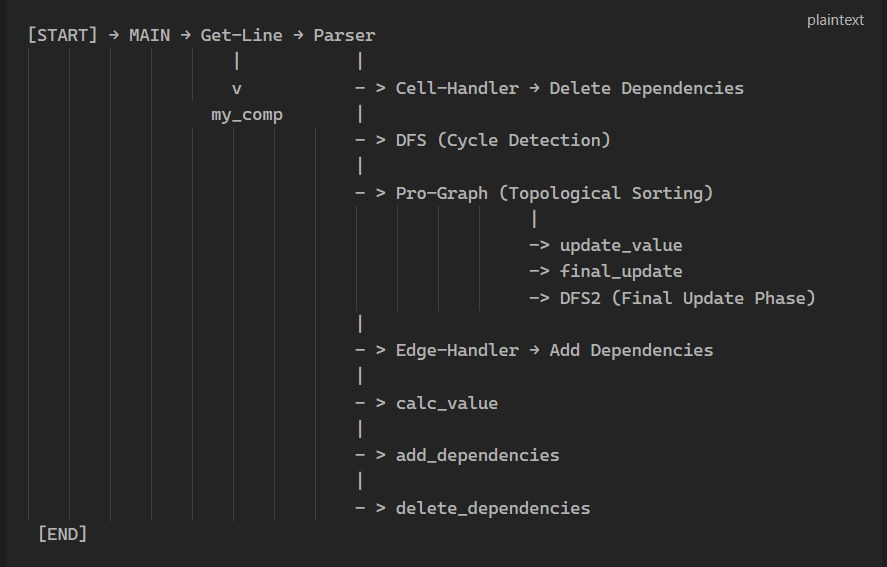
\includegraphics[width=0.3\textwidth]{copass.jpg}
\caption{\label{fig:frog}This frog was uploaded via the project menu.}
\end{figure}



\subsection{How to add Lists}

You can make lists with automatic numbering \dots

\begin{enumerate}
\item Like this,
\item and like this.
\end{enumerate}
\dots or bullet points \dots
\begin{itemize}
\item Like this,
\item and like this.
\end{itemize}


\end{document}